\chapter{Nuestra propuesta}
\label{sec:algoritmo}
\section{Agregando probabilidades a un algoritmo existente}
In this section we present a modification of the algorithm
in~\cite{arec2:2008:Areces} where the fixed order of the properties in
the input scene is replaced by a finite probability distribution.  The
required changes are fairly straightforward (see
Figures~\ref{fig:algo1} and~\ref{fig:algo2}), but the behavior of the
resulting algorithm is strikingly changed. To start with, the
algorithm is now non-deterministic: two runs of the algorithm with the
same input might result in different REs for the objects in the scene.
Putting it differently, we can now generate a distribution probability
for the REs generated by the algorithm by repeatedly running it over
the same input.  As we will empirically show in
Section~\ref{sec:evaluation}, given a corpus of REs for a given scene,
it is possible to compute a suitable probability distribution for the
probability of use of the relations in the scene, in such a way that
the probability distribution of the REs generated by the model
simulates the one found in the corpus.

We consider unary properties encoded as binary relations including one
additional `dummy' element in the model (e.g., we encode the fact that
$e_1$ is \emph{blue} saying that it is related to the dummy element by
the \emph{blue} binary relation).

%In order to understand how the algorithm works, and the differences with the original proposal, {\it MOVED we need first to introduce some 
%basic notions.  The input to the algorithm will be a relational model $\mathcal{M} = \tup{\Delta, \interp{\cdot}}$,
%where $\Delta$ is the non-empty domain of objects in the scene, and $\interp{\cdot}$ is an 
%interpretation function that assigns to all properties in the scene its intended extension.  For example, 
%the scene shown in Figure~\ref{GRE3D7-stimulus} could be represented by the model $\gM=\tup{\Delta,\interp{\cdot}}$ shown in Figure~\ref{GRE3D7-stimulus-graph}; where $\Delta = \{e_1,\ldots,e_7\}$, and $\interp{\emph{green}}$, for example, is $\{e_3,e_4,e_6\}$.}


\begin{figure}[ht]
\begin{minipage}[b]{0.45\linewidth}
\centering
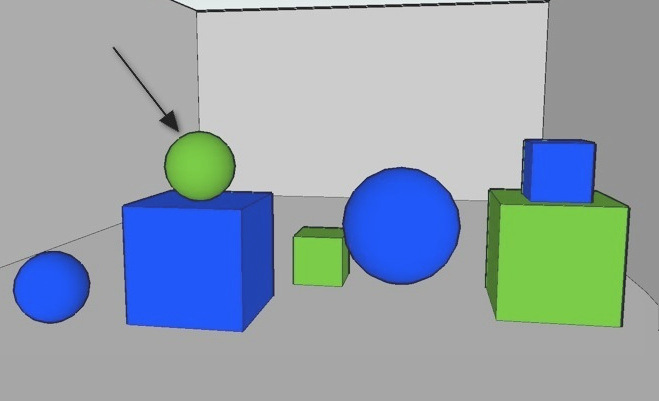
\includegraphics[width=\textwidth]{images/3.jpg}
\vspace*{.15cm}
%\caption{Input scene}
\label{GRE3D7-stimulus}
\end{minipage}
\hspace*{-0.35cm}
\begin{minipage}[b]{0.6\linewidth}
\centering
\begin{tikzpicture}
  [
    n/.style={circle,fill,draw,inner sep=3pt,node distance=1.4cm},
    aArrow/.style={->, >=stealth, semithick, shorten <= 2pt, shorten >= 2pt},
  ]
 \node[n,label=above:$e_1$,label=below:{
    \relsize{-1}$\begin{array}{c}
      \nLeft\\[-2pt]
      \nSmall\\[-2pt] 
      \nBlue \\[-2pt] 
      \nBall\end{array}$}] (a) {};

 \node[n,label=above:$e_2$,label=below:{
    \relsize{-1}$\begin{array}{c}
      \nLeft\\[-2pt]
      \nBig\\[-2pt] 
      \nBlue\\[-2pt] 
      \nCube\end{array}$}, right of=a] (b) {};

 \node[n,label=below:$e_3$,label=above:{
    \relsize{-1}$\begin{array}{c}
      \nTop\\[-2pt]
      \nLeft\\[-2pt]
      \nSmall\\[-2pt] 
      \nGreen\\[-2pt] 
      \nBall\end{array}$}, above of=b] (c) {};

 \node[n,label=above:$e_4$,label=below:{
    \relsize{-1}$\begin{array}{c}
      \nSmall\\[-2pt] 
      \nGreen\\[-2pt] 
      \nCube\end{array}$}, right of=b] (d) {};

 \node[n,label=above:$e_5$,label=below:{
    \relsize{-1}$\begin{array}{c}
      \nBig\\[-2pt] 
      \nBlue\\[-2pt] 
      \nBall\end{array}$}, right of=d] (e) {};

 \node[n,label=above:$e_6$,label=below:{
    \relsize{-1}$\begin{array}{c}
      \nBig\\[-2pt] 
      \nGreen\\[-2pt] 
      \nCube\end{array}$}, right of=e] (f) {};

 \node[n,label=below:$e_7$,label=above:{
    \relsize{-1}$\begin{array}{c}
      \nTop\\[-2pt]
      \nSmall\\[-2pt] 
      \nBlue\\[-2pt] 
      \nCube\end{array}$}, above of=f] (g) {};

 \draw [aArrow,bend right=90] (b) to node[auto,swap]{\relsize{-1}$\nBelow$} (c);
 \draw [aArrow,bend right=90] (c) to node[auto,swap]{\relsize{-1}$\nOntop$} (b);

 \draw [aArrow,bend right=30] (d) to node[auto,swap]{\relsize{-1}$\nLeftof$} (e);
 \draw [aArrow,bend right=30] (e) to node[auto,swap]{\relsize{-1}$\nRightof$} (d);

 \draw [aArrow,bend right=90] (f) to node[auto,swap]{\relsize{-1}$\nBelow$} (g);
 \draw [aArrow,bend right=90] (g) to node[auto,swap]{\relsize{-1}$\nOntop$} (f);

 \draw[dotted] (-.5,-1.4) rectangle (7.1,3.1);

 \end{tikzpicture}
\caption{Scene as a relational model}
\label{GRE3D7-stimulus-graph}
\end{minipage}
\end{figure}

%It is clear that a scene can be encoded in different ways as a relational model (for example, we could argue that $e_1$ is also \emph{leftof} $e_2$, and so on).  The algorithm assumes that these issues have been resolved and that the model encodes a suitable representation of the scene we want to describe.  Moreover, we will assume that all relations are \emph{binary}.  We will not consider relations of arity greater than two (relations of higher arity can be encoded as binary relations via reification, if necessary), and unary
%properties can be encoded as binary relations including one additional `dummy' element in the model (e.g., we encode the fact that $e_1$ is \emph{blue} saying that it is related to the dummy element by the \emph{blue} binary relation).

%On termination, the algorithm computes what are called the $\mathcal{L}$-similarity classes of the input model $\gM$. Intuitively, if two elements in the model belong to the same $\mathcal{L}$-similarity class, then $\mathcal{L}$ is not expressive enough to tell them appart (i.e, no formula in $\mathcal{L}$ can distinguish them). 

%In what follows, we will use formulas of the $\el$ description logic language~\cite{baad:desc03} to describe refinement classes.  As discussed in~\cite{arec2:2008:Areces}, this language is suitable for conjunctive relational RE, which are the ones we will find in the corpora used for our evaluation\footnote{Notice, though, that the particular formal language used is independent of the main algorithm, and different add$_{\mathcal{L}}$(R,$\varphi$,\RE) functions can be used depending on the language involved.}. For a detail description of $\el$, we refer to~\cite{baad:desc03}.  For this paper, we only need to know that the interpretation of the formula $\psi \sqcap \exists$R.$\varphi$ is the set of all elements that satisfy $\psi$ and that are related by relation R to some element that satisfy $\varphi$. For example, the interpretation of the formula \emph{ball} $\sqcap \exists$\emph{leftof}.\emph{cube} is the set of all balls that are on the left of some cube.  

We are now ready to describe Algorithms~\ref{algo:bisim-l}
and~\ref{algo:bisim-add-el}. Algorithm~\ref{algo:bisim-l} takes as
input a model $\gM$ and a list Rs of pairs (R,R.\puse) that links each
relation R to some probability of use R.\puse. I.e., if $\REL$ is the
set of all relation symbols in the model (i.e., the \emph{signature}
of the model) then Rs $\in (\REL \times [0,1])^*$. Moreover, we assume
Rs to be ordered by R.\puse.

%\begin{figure}[t]
%\small
%\centering
%\begin{algorithm}[H]
%\dontprintsemicolon
%\caption{Computing $\mathcal{L}$-similarity classes}\label{algo:bisim-l}
%\KwIn{\footnotesize A model $\gM$ and a list Rs $\in (\REL \times [0,1])^*$
% of relation symbols with their \puse\ values, ordered by \puse}
%\KwOut{\footnotesize A set of formulas \RE such that
%$\{\interp{\varphi} \mid \varphi \in \RE\}$ is the set of
%$\mathcal{L}$-similarity classes of $\gM$}

%$\RE \leftarrow \{\top\}$\tcp*[f]{\footnotesize the most general description $\top$ applies to all elements in the scene}

%\For{\em (R,R.\puse) $\in$ Rs}{
%	R.\randomuse = Random(0,1)\tcp*[f]{\footnotesize R.\randomuse is the probability of using R} \;
%        R.\incuse = (1 $-$ R.\puse) / MaxIterations\tcp*[f]{\footnotesize R.\puse\ are incremented by R.\incuse in each loop}
%}

%\Repeat{\em $\forall$((R,R.\puse) $\in$ Rs).(R.\puse $\ge$ 1)\tcp*[f]{\footnotesize R.\puse\ are incremented until they reach 1}}{
%  \While(\tcp*[f]{\footnotesize while some class has at least two elements}){\em $\exists (\varphi \in$ \RE)$.(|\interp{\varphi}|>1)$}{
%      \RE' $\leftarrow$ \RE \tcp*[f]{\footnotesize make a copy for future comparison} \;
%      \For{\em (R, R.\puse) $\in$ Rs}{
%          \If(\tcp*[f]{\footnotesize R will be used in the expression}){\em R.\randomuse $\le$ R.\puse}{
%              \For{\em $\varphi \in$ \RE}{
%                  add$_\mathcal{L}$(R, $\varphi$, \RE)\tcp*[f]{\footnotesize refine all classes using R}}
%                  }\;
%              \If(\tcp*[f]{\footnotesize the classification has changed}){\em \RE $\not =$ \RE'}{exit\tcp*[f]{\footnotesize exit for-loop to try again highest R.\puse}}
%              }
%     \If(\tcp*[f]{\footnotesize the classification has stabilized}){\em \RE $=$ \RE'}{exit\tcp*[f]{\footnotesize exit while-loop to increase R.\puse}}
%  }
%  \For{\em (R,R.\puse) $\in$ Rs}{
%    R.\puse $\leftarrow$ R.\puse $+$ R.\incuse\tcp*[f]{\footnotesize increase R.\puse}
%  }
%}
%\end{algorithm}
%\vspace*{-.5cm}\caption{Main algorithm, dealing with probabilities}\label{fig:algo1}
%\end{figure}


%\begin{figure}[t]
%\small
%\centering
%\begin{algorithm}[H]
%\dontprintsemicolon
%\caption{add$_\el$(R, $\varphi$, \RE)} \label{algo:bisim-add-el}

%\For{\em $\psi \in$ \RE with $|\interp{\psi}| > 1$}{
%  \If(\tcp*[f]{\footnotesize informative: smaller than the original?}){\em $\psi \sqcap \exists$R.$\varphi$ is not subsumed in \RE\ {\bf and} \tcp*[f]{\footnotesize non-redundant: can't be obtained from \RE?}\\
%    \em \ \ \ $\interp{\psi \sqcap \exists \mbox{\em R}.\varphi} \neq \emptyset$ {\bf and} \tcp*[f]{\footnotesize non-trivial: has elements?}\\
%     \ \ \ $\interp{\psi \sqcap \exists \mbox{\em R}.\varphi} \neq \interp{\psi}$ }{
%    add $\psi \sqcap \exists \mbox{R}.\varphi$ to $\RE$ \tcp*[f]{\footnotesize add the new class to the classification} \;
%    remove subsumed formulas from $\RE$ \tcp*[f]{\footnotesize remove redundant classes}
%  }
%}
%\end{algorithm}
%\vspace*{-.5cm}\caption{Refinement function for the \el-language}\label{fig:algo2}
%\end{figure}

The set $\RE$ will contain the formal description of the refinement
classes and it is initialized by the most general description $\top$.
For each R, we first compute R.\randomuse, a random number in [0,1].
If R.\randomuse $\le$ R.\puse\ then we will use R to refine the set of
classes.  The value of R.\puse\ will be incremented by $R.\incuse$ in
each main loop, to ensure that all relations are, at some point,
considered by the algorithm.  This ensures that a referring expression
will be found if it exist; but gives higher probability to expressions
using relations with a high R.\puse.
 
While $\RE$ contains descriptions that can be refined (i.e., classes
with at least two elements) we will call the refinement function
add$_\mathcal{L}$(R,$\varphi$,$\RE$) successively with each relation
in Rs. A change in one of the classes, can trigger changes in
others. For that reason, if $\RE$ changes, we exit the for-loop to
start again with the relations of higher R.\puse. If the after trying
to refine the set with all relations in Rs, the set $\RE$ has not
changed, the we have reach a stable state (i.e., the classes described
in $\RE$ cannot be further refined, using the current R.\puse\
values). We will then increment all the R.\puse\ values and start the
procedure again.

Algorithm~\ref{algo:bisim-add-el} coincides with the one described
in~\cite{arec2:2008:Areces}.  It will refine each of the descriptions
in $\RE$ using the relation R and the other descriptions already in
$\RE$, under certain conditions. The new description should be
\emph{non-redundant} (the new class cannot be obtained as the union of
classes already represented in $\RE$), \emph{non-trivial} (the new
class is not empty), and \emph{informative} (the new class should not
coincide with the original class).  If all this conditions are met,
the new description is added to $\RE$, and redundant descriptions
possible created by the addition of the new description are
eliminated.

Suppose fixed an input model $\gM$ and values for Rs, and fix also
some target element $t$.  Assume also that $t$ indeed has an
$\el$-referring expression.  Upon termination,
Algorithm~\ref{fig:algo1} will compute an $\el$ formula $\varphi$ such
that $\interp{\varphi} = \{t\}$, but $\varphi$ might be different in
each run of the algorithm (even though $\gM$ and Rs are fixed).  If we
repeat this experiment a statistically significant number of times, we
can define an estimate of the probability distribution of the REs
generated by the algorithm for $t$, given $\gM$ and Rs. In
Section~\ref{sec:evaluation} we will show that given a corpus of REs
for $\gM$, it is possible to define R.\puse\ values so that this
probability distribution matches with good accuracy the probability
distribution of REs found in the corpus.

\subsection{Learning to describe new objects from corpora}
\label{sec:learning}

In the previous section we presented an algorithm that assumes that
each relation R used in a referring expressions has a known
probability of use R.\puse. In this section, we describe how to
calculate these probabilities from corpora.  The general set up is the
following: we assume available a corpus of REs associated to different
scenes that are typical of the domain in which the GRE algorithm will
have to operate.  We show first how to calculate R.\puse\ values for
those scenes for which a corpus of REs is available.  We then show how
to generalize these values to other scenes in the domain, using a
machine learning algorithm. \textit{First we} will exemplify the
methodology using the GRE3D7 corpus which we introduce in the Section
~\ref{sec:learningGRE} and then we will show how to do the same with
the TUNA-corpus that we describe in Section~\ref{sec:learningTUNA}.

\subsubsection{Calculating \puse\ when a corpus for the scene is available}

Suppose we want to automatically generate REs for target $t$ in a
given scene, and that we do have available a corpus $C$ of REs for $t$
in that scene (this is exactly the kind of information we find in the
GRE3D7 corpus \textit{and in the TUNA-corpus}).  We use the REs in $C$
to define the relational model used by the algorithm.  Then we
estimate the value of \puse\ for each of the relations in the model as
the percentage of REs in which the relation appears.  I.e.,
\begin{equation}\label{eq1}
R.\puse = \frac{\# \mbox{ of REs in $C$ in which R appears}}{\# \mbox{ of REs in $C$}}.
\end{equation}

In the case of the TUNA corpus the calculation is not neccesary
because we have only one RE for each scene.

This estimation is overly simplified and, for example, it does not
differentiate between the properties of a target and the properties of
a landmark object used in a relational RE to complete the description
of the target.  But it is extremely easy to compute, and we will see
in Section~\ref{sec:evaluation} that it already produces natural REs
that match those found in the corpus.

To clarify the computation of R.\puse\ and the model $\gM$ associated
to each scene we list the required steps in detail, and discuss how we
carried them out in the GRE3D7 corpus:

\begin{enumerate}
\item Tokenize the referring expressions and call the set of tokens
  $T$. In particular, multi-word expressions like ``on top of''
  should be matched to a single token like \emph{ontop}.

\item Remove hyperonyms from $T$. E.g., if both \emph{cube} and
  \emph{thing} appear in $T$, delete \emph{thing}.

\item If the set of tokens obtained in the previous steps contains
  synonyms normalize them to a representative in the synonym class,
  and call the resulting set $\REL$; it will be the signature of the
  model $\gM$ used by the algorithm. E.g., the tokens \emph{little}
  and \emph{small} are both represented by the token \emph{small}.

\item For each scene, define $\gM$ such that the interpretation
  $\interp{\cdot}$ ensures that all the REs in the corpus are REs in
  the model.  E.g., the $\el$ formulas corresponding to the REs in
  Table~\ref{corpus-distribution} should all denote the target in the
  model $\gM$ depicted in
  Figure~\ref{GRE3D7-stimulus-graph}.

\item For each R $\in \REL$ compute R.\puse\ using~(\ref{eq1}) if we
  ave many RE for each scene or we assign 1 to R.\puse\ if R occurs in
  the RE, we assign 0 otherwise.

\end{enumerate}

Steps 1-5 above are easy to carry out (actually, the tokenization and
normalization steps were already done in the GRE3D7 corpus).  Starting
from the scene in Figure~\ref{GRE3D7-stimulus} and the corresponding
corpus shown in Table~\ref{corpus-distribution}, the resulting
signature and their associated \puse\ are listed in the first three
columns of Table~\ref{probability-of-use}.

Notice that the values R.\puse\ obtained in this way should be
interpreted as the probability of using R to describe the target in
model $\gM$, and we could argue that they are correlated to the
\emph{saliency} of R in the model.  For that reason, for example, the
value of \emph{ball}.\puse\ is 1, while the value of
\emph{cube}.\puse\ is 0.178.  These probabilities will not be useful
to describe different targets in different scenes.  We will see how we
can use them to obtain values for new targets and scenes using a
machine learning approach in the next section.  Not surprisingly,
using these values for R.\puse\ the REs generated most often by the
algorithm can be found in the corpus.  More interestingly, as we
discuss in Section~\ref{sec:evaluation} the algorithm generates REs
with a distribution that matches the one found in the corpus and, as
Table~\ref{results-algo-fig3} shows, even the generated REs not found
in the corpus are natural.


\subsubsection{Calculating \puse\ for scenes without corpora for the
  target} \label{subsec:learning}

If there is no corpora that describes the target we can estimate the
\puse~from corpora on a different scenes in the same domain.

We use simple features to obtain the function, all the features can be
extracted automatically from the relational model and are listed in
Table~\ref{features}.

\begin{small}
\begin{table}[h!]
\begin{center}
\begin{tabular}{|l|p{10cm}|}
\hline
target & whether the target element has the property. \\
\#rel-prop & number of properties and relations that the target has.\\
\#rel & number of the relations that the target has. \\
landmark & whether a landmark of the target has the property, an object is a landmark if there is a direct relation in the model 
between them (for the GRE3D7).\\
location-has & whether the RE may use the location of the target in the figure (for TUNA corpus).\\
discrimination & 1 over the number of objects in the model that have the property.  \\
\hline
\end{tabular}
\caption{Features used for learning the \puse ~for each token in the signature of the scenes \textit{(GRE3D7 and TUNA-corpus)} \label{features}}
\end{center}
\end{table}
\end{small}

Our feature set is intentionally simplistic in order for it to be
domain independent. As a result there are some complex relations
between characteristics of the scenes that it is not able to
capture. The most important characteristic of the GRE3D7 domain is
that we are not able to learn, and has an impact in our performance,
the properties of type size (namely, small and large) are used much
more when the target cannot be uniquely identified with taxonomical
(ball and cube) and absolute (green and blue) properties only.  In
other words, in the GRE3D7 corpus the size is used more often (90.2\%)
of the time when the resulting RE is not overspecified than when it is
(34\%). It may not be possible to learn this characteristic from the
GRE3D7 data since even with the domain dependent features defined
in~\cite[Chapter 6]{viet:gene11}, it could not be learned by decision
trees. As a result we can see in Table~\ref{probability-of-use} that
for Fig 13 the value estimated for ``large'' are not close to the
value calculated from corpora.  \textit{In the case of the TUNA-corpus
  we show that we couldn't learn the dependency of dimension-x and
  dimension-y, it mean, when a person adds dimension-x is highly
  probably that he includes dimension-y in his referring expression.}

\begin{table}[h!]
\begin{center}
\begin{tabular}{|l|c|c|c|c|}
\hline
Token & Model Fig 3 \puse & Learned Fig 3\puse & Model Fig 13 \puse & Learned Fig 13 \puse \\
\hline
ball & 1.0 & 1.0 & 1.0 & 1.0 \\
cube & 1.0 & 1.0 & 1.0 & 1.0 \\
green & 0.978 & 0.993 & 1.0 & 0.9875 \\
small & 0.257 & 0.346 & 0.0428 & 0.1993 \\
on-top & 0.178 & 0.179 & 0 & 0\\ 
blue & 0.15 & 0.124 & 0.064 & 0.1353 \\
large & 0.107 & 0.03 & 0.307 & 0.7378 \\
left & 0.007 & 0.002 & 0 & 0.0024 \\
top & 0.007 & 0 & 0 & 0 \\
right & 0 & 0.001 & 0.064 & 0.0005 \\
left-of & 0 & 0 & 0 & 0 \\
right-of & 0 & 0 & 0.064 & 0.1023 \\
below-of & 0 & 0 & 0 & 0 \\
\hline
\end{tabular}
\caption{Probabilities of use of the tokens from the corpora in Table~\ref{GRE3D7-stimulus}  \textit{(GRE3D7)} \label{probability-of-use}}
\end{center}
\end{table}

The learning was done with the machine learning toolkit
WEKA~\cite{Hall:WEK09}, training on all minus one (the one for that we
are learning) for all the scenes of the GRE3D7 \textit{and the
  TUNA-corpus}.  We use linear regression to learn the function of
\puse\ for each word in the signature.  For a given scene, we replace
the variables of the obtained function by the values of the features
in the scene that we want to describe.

Using linear regression we are able to learn interesting
characteristics of the domain. To start with, it learns known facts
such that the saliency of a color depends strongly on whether the
target object is of that color, and it does not depend on its
discrimination power in the model. Moreover, it learns that the on-top
relation is used more frequently than the horizontal relations
(left-of and right-of) which confirms a previous finding reported
in~\cite{viet:gene11}. Finally, it learned a surprising fact of the
GRE3D7 corpus (not found by previous work), that is that size is used
more frequently in an overspecified manner when the target and
landmark share the size. Size was used in overspecified REs in 49\% of
the descriptions for scenes where target and landmark shared the size,
and 25\% of the time when target and landmark did not share the
size. This can be explained by the observation that if landmark and
target share a property, this property is more salient.



\subsection{Generating overspecified descriptions}\label{sec:overspecification}

As it stand, Algorithm~\ref{algo:bisim-l} allows very little overspecification in the REs it
generates.  A relation with a low \puse\ might be enough 
(by itself or in combination with some of the relations already considered) to 
identify the target. Once this relation is added, we obtain an RE, but a shorter, 
more specific RE might be possible, by eliminating some of the previous refinements. 
Hence, the resulting RE might be overspecified. This is the same kind of overspecification 
that the original incremental algorithm allows.  But it has been argued~\cite{Engelhardt_Bailey_Ferreira_2006,Arts_Maes_Noordman_Jansen_2011} that 
a much higher degree of overspecification is usually found in corpora, and this 
is indeed what can be seen in the GRE3D7 corpus.  As we can see in Table~\ref{corpus-distribution}, 
the target is described 16.43\% of the times as a ``small green ball'' when ``green 
ball'' is already an RE.  Using the \puse\ values learnt from the calculus explained
in the previous section, Algorithm~\ref{algo:bisim-l} cannot simulate this behavior. 

Because the fundamental idea of the algorithm is semantics, handling overspecification in 
a natural way is difficult. If two properties have the same interpretation in a given 
model, then once the first has been considered the second will not refine the classes 
obtained so far, and hence the algorithm won't include it in the generated descriptions. 
On the other hand, if we disregard the condition the informativeness constrain (i.e., 
the fact that the addition of a relation indeed refine the class, eliminating some of 
the elements it contains), then we run the risk of generating descriptions like ``the green 
green ball.''

As a compromise, we consider the following variation of Algorithm~\ref{algo:bisim-l} were 
we disregard the informativeness constrain (i.e., we allow the inclusion of new relations 
in the description, even if they do not refine the associated class) \emph{but only during the 
first loop of the algorithm}.  That is, during the first loop over the elements in the 
input list Rs, we will allow the inclusion of all relations that do not trivialize the 
description (i.e., the associated class is not empty).  Because this is done only during 
the first loop, we know that repeated properties will not appear in the generated REs.  
In the remaining loops, additional properties will be added only if they are informative. 
%The modified algorithm is shown in Figure~\ref{fig:algo3}.

%%\newcommand{\nBlue}{\mathit{blue}\xspace}
%%\newcommand{\nGreen}{\mathit{green}\xspace}
%%\newcommand{\nSmall}{\mathit{small}\xspace}
%%\newcommand{\nBig}{\mathit{big}\xspace}
%%\newcommand{\nBall}{\mathit{ball}\xspace}
%%\newcommand{\nCube}{\mathit{cube}\xspace}
%%\newcommand{\nOntop}{\mathit{ontop}\xspace}
%%\newcommand{\nTop}{\mathit{top}\xspace}
%%\newcommand{\nBelow}{\mathit{below}\xspace}
%%\newcommand{\nRightof}{\mathit{rightof}\xspace}
%%\newcommand{\nLeftof}{\mathit{leftof}\xspace}
%%\newcommand{\nLeft}{\mathit{left}\xspace}

%\begin{figure}[ht]
%\begin{minipage}[b]{0.42\linewidth}
%\centering
%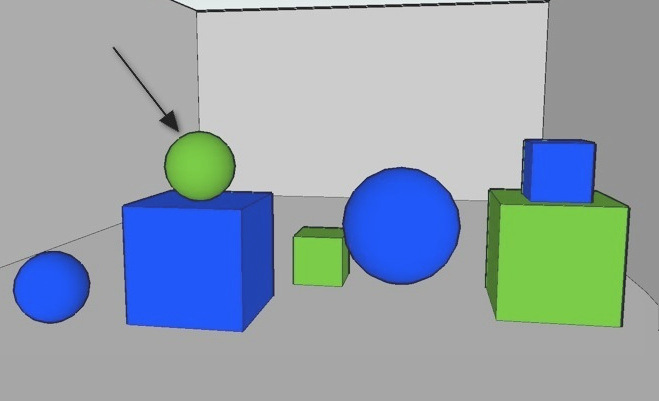
\includegraphics[width=\textwidth]{images/3.jpg}
%\vspace*{-.25cm}
%\vspace*{-.4cm}\caption{Input scene}
%\label{GRE3D7-stimulus}
%\end{minipage}
%\hspace*{-0.2cm}
%\begin{minipage}[b]{0.6\linewidth}
%\centering
%\begin{tikzpicture}
%  [
%    n/.style={circle,fill,draw,inner sep=3pt,node distance=1.4cm},
%    aArrow/.style={->, >=stealth, semithick, shorten <= 2pt, shorten >= 2pt},
%  ]
% \node[n,label=above:$e_1$,label=below:{
%    \relsize{-1}$\begin{array}{c}
%      \nLeft\\[-2pt]
%      \nSmall\\[-2pt] 
%      \nBlue \ \  
%      \nBall\end{array}$}] (a) {};

% \node[n,label=above:$e_2$,label=below:{
%    \relsize{-1}$\begin{array}{c}
%      \nLeft\\[-2pt]
%      \nBig\\[-2pt] 
%      \nBlue \ \  
%      \nCube\end{array}$}, right of=a] (b) {};

% \node[n,label=below:$e_3$,label=above:{
%    \relsize{-1}$\begin{array}{c}
%      \nTop \ \       \nLeft \ \ 
%      \nSmall \ \       \nGreen \ \ 
%      \nBall\end{array}$}, above of=b] (c) {};

% \node[n,label=above:$e_4$,label=below:{
%    \relsize{-1}$\begin{array}{c}
%      \nSmall\\[-2pt] 
%      \nGreen\\[-2pt] 
%      \nCube\end{array}$}, right of=b] (d) {};

% \node[n,label=above:$e_5$,label=below:{
%    \relsize{-1}$\begin{array}{c}
%      \nBig\\[-2pt] 
%      \nBlue\\[-2pt] 
%      \nBall\end{array}$}, right of=d] (e) {};

% \node[n,label=above:$e_6$,label=below:{
%    \relsize{-1}$\begin{array}{c}
%      \nBig\\[-2pt] 
%      \nGreen\\[-2pt] 
%      \nCube\end{array}$}, right of=e] (f) {};

% \node[n,label=below:$e_7$,label=above:{
%    \relsize{-1}$\begin{array}{c}
%      \nTop \ \ 
%      \nSmall\ \ 
%      \nBlue \ \  
%      \nCube\end{array}$}, above of=f] (g) {};

% \draw [aArrow,bend right=90] (b) to node[auto,swap]{\relsize{-1}$\nBelow$} (c);
% \draw [aArrow,bend right=90] (c) to node[auto,swap]{\relsize{-1}$\nOntop$} (b);

% \draw [aArrow,bend right=30] (d) to node[auto,swap]{\relsize{-1}$\nLeftof$} (e);
% \draw [aArrow,bend right=30] (e) to node[auto,swap]{\relsize{-1}$\nRightof$} (d);

% \draw [aArrow,bend right=90] (f) to node[auto,swap]{\relsize{-1}$\nBelow$} (g);
% \draw [aArrow,bend right=90] (g) to node[auto,swap]{\relsize{-1}$\nOntop$} (f);

% \draw[dotted] (-.65,-1.2) rectangle (7.1,2.1);

% \end{tikzpicture}
%\vspace*{-.4cm}\caption{Scene as a relational model}
%\label{GRE3D7-stimulus-graph}
%\end{minipage}
%\end{figure}

On termination, the algorithm computes what are called the $\mathcal{L}$-similarity classes of the input model $\gM$. Intuitively, if two elements in the model belong to the same $\mathcal{L}$-similarity class, then $\mathcal{L}$ is not expressive enough to tell them appart (i.e, no formula in $\mathcal{L}$ can distinguish them). 

The algorithm we discuss uses formulas of the $\el$ description logic language~\cite{baad:desc03} to describe refinement classes\footnote{Notice, though, that the particular formal language used is independent of the main algorithm, and different add$_{\mathcal{L}}$(R,$\varphi$,\RE) functions can be used depending on the language involved.}. 
For a detailed description of $\el$, we refer to~\cite{baad:desc03}.  
The interpretation of the $\el$ formula $\psi \sqcap \exists$R.$\varphi$ is the set of all elements that satisfy $\psi$ and that are related by relation R to some element that satisfy $\varphi$. 
For example, the interpretation of the formula \emph{ball} $\sqcap \exists$\emph{leftof}.\emph{cube} is the set of all balls that are on the left of some cube.  

%%We are now ready to describe Algorithms~\ref{algo:bisim-l} and~\ref{algo:bisim-add-el-over}. 

%\begin{figure}[!t]
%\small
%\centering
%\begin{algorithm}[H]
%\dontprintsemicolon
%\caption{Computing $\mathcal{L}$-similarity classes}\label{algo:bisim-l}
%\KwIn{\footnotesize A model $\gM$ and a list Rs $\in (\REL \times [0,1])^*$
% of relation symbols with their \puse\ values, ordered by \puse}
%\KwOut{\footnotesize A set of formulas \RE such that
%$\{\interp{\varphi} \mid \varphi \in \RE\}$ is the set of
%$\mathcal{L}$-similarity classes of $\gM$}

%$\RE \leftarrow \{\top\}$\tcp*[f]{\footnotesize the most general description $\top$ applies to all elements in the scene}

%\For{\em (R,R.\puse) $\in$ Rs}{
%	R.\randomuse = Random(0,1)\tcp*[f]{\footnotesize R.\randomuse is the probability of using R} \;
%        R.\incuse = (1 $-$ R.\puse) / MaxIterations\tcp*[f]{\footnotesize R.\puse\ are incremented by R.\incuse in each loop}
%}

%\Repeat{\em $\forall$((R,R.\puse) $\in$ Rs).(R.\puse $\ge$ 1)\tcp*[f]{\footnotesize R.\puse\ are incremented until they reach 1}}{
%  \While(\tcp*[f]{\footnotesize while some class has at least two elements}){\em $\exists (\varphi \in$ \RE)$.(\#\interp{\varphi}>1)$}{
%      \RE' $\leftarrow$ \RE \tcp*[f]{\footnotesize make a copy for future comparison} \;
%      \For{\em (R, R.\puse) $\in$ Rs}{
%          \If(\tcp*[f]{\footnotesize R will be used in the expression}){\em R.\randomuse $\le$ R.\puse}{
%              \lFor{\em $\varphi \in$ \RE}{
%                  add$_\mathcal{EL}$(R, $\varphi$, \RE)\tcp*[f]{\footnotesize refine all classes using R}}
%                  }\;
%              \If(\tcp*[f]{\footnotesize the classification has changed}){\em \RE $\not =$ \RE'}{exit\tcp*[f]{\footnotesize exit for-loop to try again highest R.\puse}}
%              }
%     \If(\tcp*[f]{\footnotesize the classification has stabilized}){\em \RE $=$ \RE'}{exit\tcp*[f]{\footnotesize exit while-loop to increase R.\puse}}
%  }
%  \lFor{\em (R,R.\puse) $\in$ Rs}{
%    R.\puse $\leftarrow$ R.\puse $+$ R.\incuse\tcp*[f]{\footnotesize increase R.\puse}
%  }
%}
%\end{algorithm}

%\begin{algorithm}[H]
%\dontprintsemicolon
%\caption{add$_\el$(R, $\varphi$, \RE)} \label{algo:bisim-add-el-over}


%\begin{figure}[t]
%\small
%\centering
%\begin{algorithm}[H]
%\dontprintsemicolon
%\caption{add$_\el$(R, $\varphi$, \RE)} \label{algo:bisim-add-el-over}

%\If(\tcp*[f]{\footnotesize are we in the first loop?}){\em FirstLoop?}{
%    Informative $\leftarrow$ TRUE \tcp*[f]{\footnotesize allow overspecification}}
%\lElse(\tcp*[f]{\footnotesize informative: smaller than the original?}) {Informative $\leftarrow$ $\interp{\psi \sqcap \exists \mbox{\em R}.\varphi} \neq \interp{\psi}$} 
%\For{\em $\psi \in$ \RE with $\#\interp{\psi} > 1$}{
%  \If{\em $\psi \sqcap \exists$R.$\varphi$ is not subsumed in \RE\ {\bf and} \tcp*[f]{\footnotesize non-redundant: can't be obtained from \RE?}\\
%    \em \ \ \ $\interp{\psi \sqcap \exists \mbox{\em R}.\varphi} \neq \emptyset$ {\bf and} \tcp*[f]{\footnotesize non-trivial: has elements?}\\
%     \ \ \  \emph{Informative}}{
%    add $\psi \sqcap \exists \mbox{R}.\varphi$ to $\RE$ \tcp*[f]{\footnotesize add the new class to the classification} \;
%    remove subsumed formulas from $\RE$ \tcp*[f]{\footnotesize remove redundant classes}
%  }
%}
%\end{algorithm}
%\vspace*{-.5cm}\caption{Refinement algorithm with probabilities and overspecification for the \el-language}\label{fig:algo3}

%\end{figure}

Algorithm~\ref{algo:bisim-l} takes as input a model and a list Rs of pairs (R,R.\puse) that links each relation R $\in \REL$, the set of all relation symbols in the model,  to some probability of use R.\puse. 
I.e., if $\REL$ is the set of all relation symbols in the model then Rs $\in (\REL \times [0,1])^*$. We assume Rs to be ordered by R.\puse. 

The set $\RE$ will contain the formal description of the refinement classes and it is initialized by the most general description $\top$.  
For each R, we first compute R.\randomuse, a random number in [0,1].  If R.\randomuse $\le$ R.\puse\ then we will use R to refine the set of classes.  The value of R.\puse\ will be incremented by R.$\incuse$ in each main loop, to ensure that all relations are, at some point, considered by the algorithm.  This ensures that a referring expression will be found if it exists; but gives higher probability to expressions using relations with a high R.\puse. 

While $\RE$ contains descriptions that can be refined (i.e., classes with at least two elements) we will call the refinement function add$_\mathcal{L}$(R,$\varphi$,$\RE$) successively with each relation in Rs. A change in one of the classes, can trigger changes in others. For that reason, if $\RE$ changes, we exit the \textbf{for} loop to start again with the relations of higher R.\puse. If after trying to refine the set with all relations in Rs, the set $\RE$ has not changed, then we have reached a stable state (i.e., the classes described in $\RE$ cannot be further refined with the current R.\puse\ values). We will then increment all the R.\puse\ values and start the procedure again. 

Algorithm~\ref{fig:algo1} almost coincides with the one in~\cite{arec2:2008:Areces}.  The \textbf{for} loop will refine each descriptions in $\RE$ using the relation R and the other descriptions already in $\RE$, under certain conditions. The new description should be \emph{non-redundant} (it cannot be obtained from classes already in $\RE$), \emph{non-trivial} (it is not empty), and \emph{informative} (it does not coincide with the original class).  If these conditions are met, the new description is added to $\RE$, and redundant descriptions created by the new description are eliminated. The \textbf{if} statement at the beginning of Algorithm in Figure~\ref{fig:algo2} disregards the informativity test during the first loop of the algorithm allowing overspecification.    

Suppose fixed an input model $\gM$ and values for Rs, and fix also some target element $t$.  Assume also that $t$ indeed has an $\el$-referring expression.  Upon termination, Algorithm~\ref{fig:algo1} will compute an $\el$ formula $\varphi$ such that $\interp{\varphi} = \{t\}$, but $\varphi$ might be different in each run of the algorithm (even though $\gM$ and Rs are fixed).  If we repeat this experiment a statistically significant number of times, we can define an estimate of the probability distribution of the REs generated by the algorithm for $t$, given $\gM$ and Rs. In Section~\ref{sec:evaluation} we will show that given a corpus of REs for $\gM$, it is possible to define R.\puse\ values so that this probability distribution matches with good accuracy the probability distribution of REs found in the corpus.  



\section{Aprendizaje autom�tico}

\section{Agregando sobreespecificaci�n}
